\label{sec:intro}


%\todo{introduce the task of 3d detection on point cloud and its importance}

Recently, great progress has been made on 2D image understanding tasks, such as object detection~\cite{girshick2014rich} and instance segmentation~\cite{he2017mask}. However, beyond getting 2D bounding boxes or pixel masks, \emph{3D understanding} is eagerly in demand in many applications such as autonomous driving and augmented reality (AR). With the popularity of 3D sensors deployed on mobile devices and autonomous vehicles, more and more 3D data is captured and processed. In this work, we study one of the most important 3D perception tasks -- 3D object detection, which classifies the object category and estimates \emph{oriented 3D bounding boxes} of physical objects from 3D sensor data. 

%\todo{representation is important for 3d detection. introduce pointnet.}

%In contrast to images with a dominant representation as 2D arrays, 3D data has many representations and each representation corresponds to a different family of deep net architectures.
While 3D sensor data is often in the form of point clouds, how to represent point cloud and what deep net architectures to use for 3D object detection remains an open problem. Most existing works convert 3D point clouds to images by projection~\cite{su15mvcnn,qi2016volumetric} or to volumetric grids by quantization~\cite{wu20153d,maturana2015voxnet,qi2016volumetric} and then apply convolutional networks. This data representation transformation, however, may obscure natural 3D patterns and invariances of the data. %MV3D~\cite{cvpr17chen} projects LiDAR point cloud into bird's eye view image, use multiple image channels to represent height information and use 2D region proposal network on the projected image. Song et al.~\cite{song2015sun} quantitizes point cloud to volumetric grids, compute distance field as voxel channels, and extends 2D region proposal networks with 3D CNNs.
% However, in conversion they all suffer from loss in 3D geometry in trade of the feasibility to apply convolutional networks, which requires data in a regular grid structure. 
Recently, a number of papers have proposed to process point clouds directly without converting them to other formats. For example, \cite{qi2017pointnet, qi2017pointnetplusplus} proposed new types of deep net architectures, called \emph{PointNets}, which have shown superior performance and efficiency in several 3D understanding tasks such as object classification and semantic segmentation.

%\todo{challenges for applying 3d deep learning to 3d detection -- proposal. how we dealt with it with our pipeline.}
\begin{figure}[t!]
    \centering
    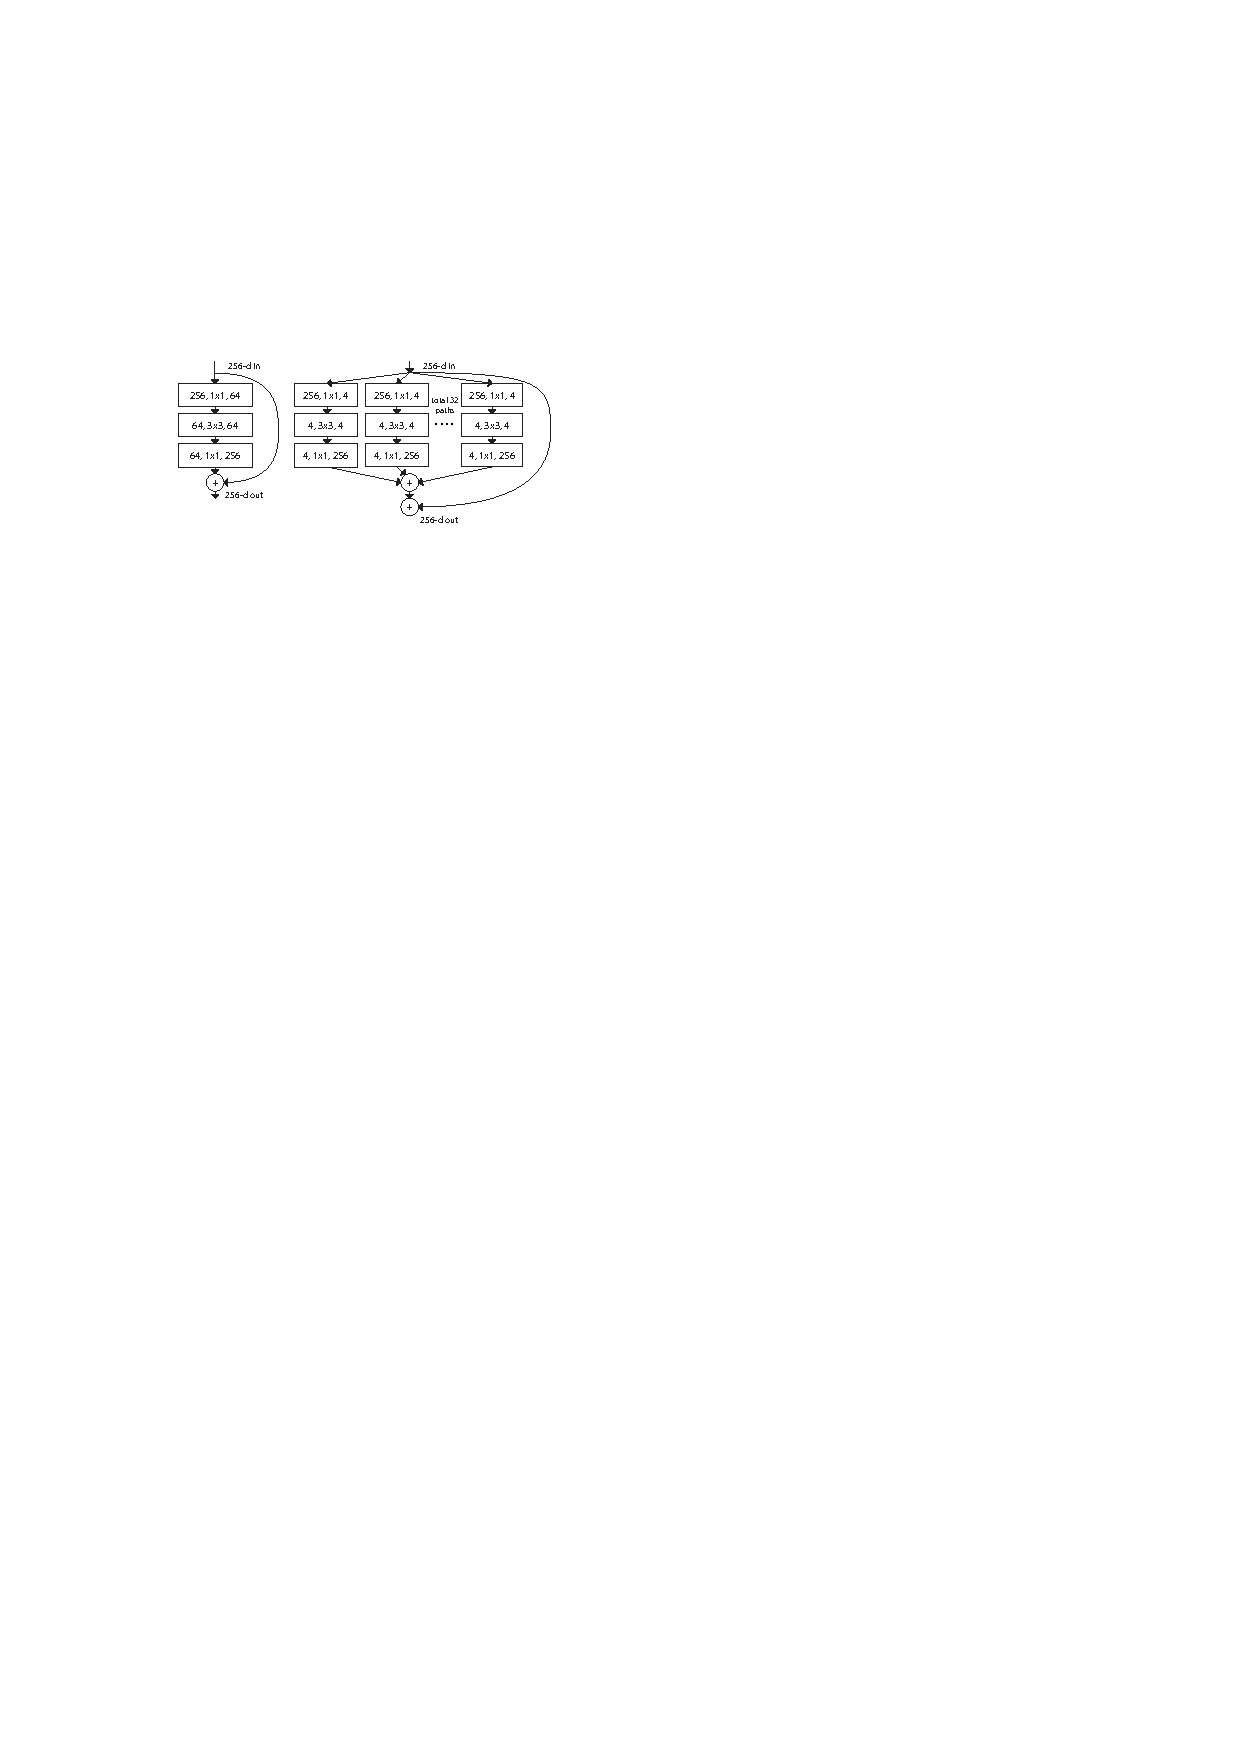
\includegraphics[width=\linewidth]{fig/teaser.pdf}
    \caption{\textbf{3D object detection pipeline.} Given RGB-D data, we first generate 2D object region proposals in the RGB image using a CNN. Each 2D region is then extruded to a \emph{3D viewing frustum} in which we get a point cloud from depth data. Finally, our frustum PointNet predicts a (oriented and amodal) 3D bounding box for the object from the points in frustum.}
    \label{fig:teaser}
\end{figure}

While PointNets are capable of classifying a whole point cloud or predicting a semantic class for each point in a point cloud, it is unclear how this architecture can be used for instance-level 3D object detection. Towards this goal, we have to address one key challenge: how to efficiently propose possible locations of 3D objects in a 3D space. Imitating the practice in image detection, it is straightforward to enumerate candidate 3D boxes by sliding windows~\cite{engelcke2017vote3deep} or by 3D region proposal networks such as \cite{song2015sun}. However, the computational complexity of 3D search typically grows cubically with respect to resolution and becomes too expensive for large scenes or real-time applications such as autonomous driving. % ; besides, it's hard to leverage RGB information for 3D search.

Instead, in this work, we reduce the search space following the dimension reduction principle: we take the advantage of mature 2D object detectors (Fig.~\ref{fig:teaser}). First, we extract the 3D bounding frustum of an object by extruding 2D bounding boxes from image detectors. Then, within the 3D space trimmed by each of the 3D frustums, we consecutively perform 3D object instance segmentation and \emph{amodal} 3D bounding box regression using two variants of PointNet. The segmentation network predicts the 3D mask of the object of interest (i.e. instance segmentation); and the regression network estimates the amodal 3D bounding box (covering the entire object even if only part of it is visible).

In contrast to previous work that treats RGB-D data as 2D maps for CNNs, our method is more \emph{3D-centric} as we lift depth maps to 3D point clouds and process them using 3D tools. This 3D-centric view enables new capabilities for exploring 3D data in a more effective manner. First, in our pipeline, a few transformations are applied successively on 3D coordinates, which align point clouds into a sequence of more constrained and canonical frames.
These alignments factor out pose variations in data, and thus make 3D geometry pattern more evident, leading to an easier job of 3D learners.
%After the alignment, the job of 3D learners becomes easier since pose variations have been factored out and 3D geometry patterns become more evident.
Second, learning in 3D space can better exploits the geometric and topological structure of 3D space.
% using specifically tailored machine learning tools such as PointNet.
In principle, all objects live in 3D space; therefore, we believe that many geometric structures, such as repetition, planarity, and symmetry, are more naturally parameterized and captured by learners that directly operate in 3D space. %Compared with 2D detection that use CNN on \emph{regions} of pixels, our 3D detection system uses PointNet on \emph{frustums} of point clouds extruded from 2D regions. %
The usefulness of this 3D-centric network design philosophy has been supported by much recent experimental evidence.
% \hao{to be rewritten}  steps play a key role, among them some are parameter-free and some are network based. The coordinate transformations helps to align point cloud into more constrained distribution space, which are critical for successful weight sharing. Besides, we also design a novel regularization loss for 3D box regression (the corner loss), which helps to jointly optimize location, size and orientation estimation of the 3D boxes.

Our method achieve leading positions on KITTI 3D object detection~\cite{kitti-3d-detection} and bird's eye view detection~\cite{kitti-3d-localization} benchmarks.
Compared with the previous state of the art~\cite{cvpr17chen}, our method is \emph{8.04\%} better on 3D car AP with high efficiency (running at 5 fps). Our method also fits well to indoor RGB-D data where we have achieved \emph{8.9\%} and \emph{6.4\%} better 3D mAP than ~\cite{lahoud20172d} and ~\cite{ren2016three} on SUN-RGBD while running one to three orders of magnitude faster.

% Therefore we call our network for 3D object detection as \emph{Frustum-based PointNet}. 



The key contributions of our work are as follows:
\bitem
    \item We propose a novel framework for RGB-D data based 3D object detection called Frustum PointNets.
    \item We show how we can train 3D object detectors under our framework and achieve state-of-the-art performance on standard 3D object detection benchmarks.
    \item We provide extensive quantitative evaluations to validate our design choices as well as rich qualitative results for understanding the strengths and limitations of our method.
\eitem

%\rqi{Our pipeline is a generalized framework that supports both front-view RGB image proposals and bird's eye view proposals: 2D box $\rightarrow$ 3D segmentation $\rightarrow$ 3D box. Instead of proposing 3D boxes as in Song et al. with 3D region proposal networks, which has huge search space and is very slow in run time, we reduce search space by firstly proposing 2D regions in images. Beyond MV3D that is restricted to bird's eye view (because there lacks a 3D segmentation stage), our framework can support both RGB view and bird's eye view proposal and uses a 3D deep learning network (PointNet) to process point cloud. }

%However, advancing to 3D object detection presents new challenges.In most cases both 2D RGB image and 3D point cloud are available for 3D detection problem. As image and point cloud complements each other in semantics and geometry, how to make best use of both 2D and 3D is still an open question. On the other hand, 3D object detection involves perception of 3D data such as point cloud. While almost all existing works stick with the most popular network architecture (ConvNet) on 2D images, it may not be the best choice for 3D detection.

%\todo{most existing work convert 3d point cloud to images by projections or volumetric data by quantization. however, they suffer from issues ... recently, a few papers have proposed to process point cloud directly without converting to other forms, and these frameworks have shown both superior performance and efficiency. }
%Recently, a popular trend for 3D object detection is to process point clouds as images and apply CNNs with well-engineered architectures for image classification. MV3D~\cite{cvpr17chen} projected 3D point cloud to bird's eye view and use region proposal network (similar to that used in Faster-RCNN) for 3D region proposals. VeloFCN~\cite{li2016vehicle} projected 3D point cloud to front view (similar to a depth map) and make dense box predictions with fully convolutional networks.

%\todo{we extend pointnet for instance segmentation and amodal object detection from 3d point cloud. pointnet is used for classification and segmentation. towards 3d detection, we have to address a key challenge: how to efficiently propose the possible locations of 3d objects, a.k.a. the 3d bounding cuboid proposal problem. existing work proposes b.box by 3d search, which is very expensive. }

%In this work, we propose a novel approach for 3D object detection that (1) jointly uses 2D images and 3D point clouds for 3D object localization and (2) adopts PointNet based deep networks for 3D point cloud perception. Our detection pipeline firstly uses CNNs for 2D region proposals in images and then uses PointNet~\cite{qi2017pointnet} based architecture for 3D segmentation and bounding box estimation in point clouds in the frustums culled by the 2D regions. In this way, we benefit from the rich semantics in RGB images for 2D region proposal as well as the rich geometry in point clouds for 3D bounding box estimation. On the other hand, image region proposals greatly reduce the search space for 3D instance segmentation while the rest heavy-lifting jobs are left to a specialized architecture (PointNet) on point clouds. 

%\todo{compared with most previous work that processes rgbd data by deep learning, our work which is 3d-centric has shown advantages according to experimental evaluations. in literature, many cnn based approaches have been proposed to process rgbd data, which is a 2d input of rgb and depth channels. our approach, on the contrary, lifts the rgbd image as a 3d point cloud and leverages pointnet that is powerful to exploit the embodied 3d structures. the advantage of such 3d-centric perspective is evident by our experiments, and we will provide a more in-depth discussion in the conclusion section.}


% \begin{enumerate}
%     \item motivate 3d object detection
%     \item previous methods cannot make use of RGB object detector OR do not make good use of 3D
%     \item we make use of the best from the two worlds -- 2D attention (image CNN) + 3D attention and regress 3D box in 3D space (with pointnet based architecture). how 3d attention/normalization matters. why doing inference in point cloud with pointnet is better than that with CNN on depth map or with 3D CNN on volumetric grids. -- our pointnet is learning occlusion and clutter patterns! why previous works don't take our approach, no good way to localize 3d object in frustum (a lot of occluder and clutter) -- pointnet to the rescue!
%     \item our experiment results on benchmark datasets
%     \item our model's real time capability
%     \item something more? e.g. the framework generalizes to other tasks
% \end{enumerate}

% \todo{\begin{enumerate}
%     \item CNN based results on RGB-D image
%     \item effects of quality of RGB detector
%     \item effects of sensor fusion
% \end{enumerate}}

\begin{figure*}[t!]
    \centering
    \includegraphics[width=0.92\linewidth]{fig/pipeline.pdf}
    \caption{\textbf{Frustum PointNets for 3D object detection.} We first leverage a 2D CNN object detector to propose 2D regions and classify their content. 2D regions are then lifted to 3D and thus become frustum proposals. Given a point cloud in a frustum ($n\times c$ with $n$ points and $c$ channels of XYZ, intensity etc. for each point), the object instance is segmented by binary classification of each point. Based on the segmented object point cloud ($m \times c$), a light-weight regression PointNet (T-Net) tries to align points by translation such that their centroid is close to amodal box center. At last the box estimation net estimates the amodal 3D bounding box for the object. More illustrations on coordinate systems involved and network input, output are in Fig.~\ref{fig:coordinate} and Fig.~\ref{fig:network}.}
    \label{fig:pipeline}
\end{figure*}